% % % % % % % % % % % % % % % % % % % % % % % % % % % % % % % % % % % % % % % % % % % %
%                                                                                     %
% Short Sectioned Assignment LaTeX Template Version 1.0 (5/5/12)                      %
% This template has been downloaded from: http://www.LaTeXTemplates.com               %
%                                                                                     %
% Original author:  Frits Wenneker (http://www.howtotex.com)                          %
%                                                                                     %
% Modified by: Fco Javier Sueza Rodríguez (fcosueza@disroot.org)                      %
%                                                                                     %
% Changes:                                                                            %
%	    - Custom Chapters, Sections and Subsections (titlesec package)                %
%           - Document type scrbook (oneside)                                         %
%           - Use babel-lang-spanish package and marvosym                             %
%           - Use hyperref, enumitem, tcolorbox and glossaries packages               %
%           - Use Time New Roman (mathptmx), Helvetic and Courier fonts               %
%                                                                                     %
% License: CC BY-NC-SA 3.0 (http://creativecommons.org/licenses/by-nc-sa/3.0/)        %
%                                                                                     %
% % % % % % % % % % % % % % % % % % % % % % % % % % % % % % % % % % % % % % % % % % % %

%-----------------------------------------------%
%	              Packages                  %
%-----------------------------------------------%

\documentclass[paper=a4, fontsize=11pt, oneside]{scrbook}

% ---- Text Input/Output ----- %

\usepackage[T1]{fontenc}
\usepackage[utf8]{inputenc}
\usepackage{mathptmx}
\usepackage[scaled=.92]{helvet}
\usepackage{courier}
\usepackage[indent=12pt]{parskip}

\usepackage{geometry}
\geometry{verbose,tmargin=3cm,bmargin=3cm,lmargin=2.6cm,rmargin=2.6cm}

% ---- Language ----- %

\usepackage[spanish]{babel}
\usepackage{marvosym}

% ---- Another packages ---- %

\usepackage{amsmath,amsfonts,amsthm}
\usepackage{graphics,graphicx}
\usepackage{titlesec}
\usepackage{fancyhdr}
\usepackage{tcolorbox}
\usepackage{hyperref}
\usepackage{enumitem}
\usepackage[automake]{glossaries}

%--------------------------------------------------------------------%
%                      Customizing Document                          %
%--------------------------------------------------------------------%


% ----------- Custom Chapters, Sections and Subsections -------------- %

\titleformat{\chapter}[display]
			{\bfseries\Huge}
			{Tema \ \thechapter} {0.5ex}
			{\vspace{1ex}\centering}

\titleformat{\section}[hang]
			{\bfseries\Large}
			{\thesection}{0.5em}{}

\titleformat{\subsection}[hang]
			{\bfseries\large}
			{\thesubsection}{0.5em}{}

\titleformat{\subsubsection}[hang]
			{\bfseries\large}
			{\thesubsubsection}{0.5em}{}

\hypersetup{
    colorlinks=true,
    linkcolor=black,
    urlcolor=magenta
}

% ------------------- Custom heaaders and footers ------------------- %

\pagestyle{fancyplain}

\fancyhead[]{}
\fancyfoot[L]{}
\fancyfoot[C]{}
\fancyfoot[R]{\thepage}

\renewcommand{\headrulewidth}{0pt} % Remove header underlines
\renewcommand{\footrulewidth}{0pt} % Remove footer underlines

\setlength{\headheight}{13.6pt} % Customize the height of the header

% --------- Numbering equations, figures and tables ----------------- %

\numberwithin{equation}{section} % Number equations within sections
\numberwithin{figure}{section} % Number figures within sections
\numberwithin{table}{section} % Number tables within sections

% ------------------------ New Commands ----------------------------- %

\newcommand{\horrule}[1]{\rule{\linewidth}{#1}} % Create horizontal rule command


%----------------------------------------------------------------------------------------
%	TÍTULO Y DATOS DEL ALUMNO
%----------------------------------------------------------------------------------------

\title{
\vspace{10ex}
\normalfont \normalsize
\Huge \textbf{Tarea 2: Sistemas Operativos y Software de un Sistema Informático}
}
\author{Francisco Javier Sueza Rodríguez}
\date{\normalsize\today}

%----------------------------------------------------------------------------------------
%                                     DOCUMENTO
%----------------------------------------------------------------------------------------
\begin{document}

\maketitle

\thispagestyle{empty}

\vspace{68ex}

\begin{center}
    \begin{tabular}{l l}
        \textbf{Centro}: & IES Aguadulce \\
        \textbf{Ciclo Formativo}: & Desarrollo Aplicaciones Web (Distancia)\\
        \textbf{Asignatura}: & Sistemas Informáticos\\
        \textbf{Tema}: & Tema 2 -  Software de un Sistema Informático\\
    \end{tabular}
\end{center}

\newpage

\tableofcontents

\vspace{15ex}

%\hrule

%\vspace{10ex}

%\listoffigures

\newpage

\section{Caso Práctico}
\textbf{Ada}, fundadora de la empresa AguadulSoft, ha visto una oportunidad excepcional de promocionar la empresa aprovechando una exposición temporal denominada "Historia del software: Sistemas Operativos" que se va a alojar en la localidad.

La empresa, a la que se le ha pedido colaboración, realizará un análisis de los distintos Sistemas Operativos así como de otros tipos de software que han surgido a lo largo de la historia.

También va a averiguar qué licencias se utilizan en los sistemas operativos y distintos programas que se utilizan en la actualidad.

\section{Actividades}

\subsection{Actividad  1: Tipos de Aplicaciones Informáticas}
Indica, justificando su uso, dos ejemplos de aplicaciones de propósito general y otros dos de propósito específico para cada uno de los siguientes entornos productivos:

\begin{itemize}
    \item Agencia de Viajes
    \item Agencia de Publicidad y Marketing
\end{itemize}

\subsubsection{Solución}
Estas dos empresas usaran tanto aplicaciones de propósito general como específico de su propio campo. En la siguiente lista se muestran dos ejemplos de cada tipo de software para cada una de las empresas.

\begin{itemize}
    \item \textbf{Agencia de Viajes}
    \begin{itemize}
        \item \textbf{Aplicaciones de Propósito General}
        \begin{itemize}
            \item \textbf{Hoja de Cálculo}: es muy probable que usen hojas de cálculo, ya que los viajes tienen muchos complementos y añadidos, y una hoja de cálculos será necesaria para calcular el precio final del paquete elegido por el cliente. Probablemente usen \textbf{Excel} o alguna alternativa libre como \textbf{Libreoffice Calc} o \textbf{Calc de Openoffice}.

            \item \textbf{Herramientas de Acceso de Bases de Datos}: también deberán emplear alguna herramienta de acceso y gestión de bases de datos, para poder consultar y administrar los destinos disponibles, precios, paquetes, etc...
        \end{itemize}

    \item \textbf{Aplicaciones de Propósito Específico}
    \begin{itemize}
        \item \textbf{Aplicaciones Ad-hoc Especializadas}: para la gestión de la agencia de viajes, los clientes, billetes, comunicación con terceros (hoteles, guías turísticos,..) se utilizará algún \textbf{CRM} especializado, como por ejemplo \textbf{CRM Travel}.

        \item \textbf{Herramientas de Administración de Bases de Datos}: además de un CRM, se deberá usar una bases de datos y herramientas para su administración, ya que este tipo de aplicaciones necesitan una base de datos como soporte. Así, podrá centralizarse toda la información de la empresa y permitirle al CRM hacer una gestión adecuada de toda esta información. Una de estás aplicaciones podría ser \textbf{OracleDB}, una de las más empleadas a nivel mundial, o \textbf{MySQL}, otra de la más usadas también.
    \end{itemize}

    \vspace{5ex}
    \end{itemize}

    \item \textbf{Agencia de Publicidad y Marketing}
    \begin{itemize}
        \item \textbf{Aplicaciones de Propósito General}
        \begin{itemize}
            \item \textbf{Generador de Presentación}: una herramienta necesaria para exponer información será un generador de presentación, bien para presentar la estrategia de una nueva campaña y sus elementos claves o para presentar datos relativos a una campaña ya realizar, entre otras cosas. Podrían usar \textbf{Microsoft Powerpoint}, por ejemplo.

            \item \textbf{Herramientas para la Comunicación}: seguramente también usen herramientas para la comunicación rápida y directa entre los diferentes departamentos, ya que el trabajo de esta empresa debe estar bien coordinado entre los diferentes equipos que conformen un mismo proyecto. Este software podría ser \textbf{Slack}, uno de los más usados.
        \end{itemize}

        \item \textbf{Aplicaciones de Propósito Específico}
        \begin{itemize}
            \item \textbf{Herramientas de Diseño Gráfico y Maquetación}: esta herramienta será básica para el diseño de campañas publicitarias, especialmente aquellas pensadas para cartelería o cualquier medio impreso. Uno de los más usados es \textbf{Adobe Photoshop}, aunque también podrían usar alternativas como libres como \textbf{Gimp} o \textbf{Inkscape}, o incluso usar la herramienta colaborativa \textbf{Figma}, cuyo uso se esta expandiendo recientemente.

            \item \textbf{Herramientas de Análisis de Datos}: la empresa necesitará diferentes herramientas de análisis de datos para conocer el impacto de las campañas, punto clave para saber si han tenido éxito o no. Esto requiere de herramientas que sean capaces de procesar grandes cantidades de datos, conocidas como \textbf{Big Data}. Una de las empleadas es \textbf{HubSpot}, especializada en el análisis de datos de marketing.
        \end{itemize}
    \end{itemize}
\end{itemize}

\subsection{Actividad 2: Licencias de Software}
Indica para cada una de las siguientes aplicaciones, el tipo de licencia que utiliza, intentando dar en términos generales si se trata de una licencia de software con código abierto, con código cerrado o de dominio público (sin licencia), y de manera específica la licencia exacta que utiliza.

Por ejemplo: El programa de edición de gráficos vectoriales llamado Inkscape, usa una licencia GPLv3+, que es una licencia de software con código abierto, no permisiva, de tipo copyleft fuerte (software libre).

Las aplicaciones son las siguientes:

\begin{itemize}
    \item Microsoft Office 2021.
    \item Google Chrome.
    \item VLC Media Player.
    \item Avast Free Antivirus.
    \item Adobe Acrobat Pro.
\end{itemize}

\subsubsection{Solución}
En esta actividad vamos a indicar bajo que licencia están desarrolladas diferentes aplicaciones, especificando si la licencia es libre y propietaria, así como sus principales características.

\begin{itemize}
    \item \textbf{Microsoft Office 2021}: esta suite ofimática se encuentra bajo la licencia \textbf{Microsoft CLUF}, una \textbf{licencia propietaria} de tipo \textbf{EULA}, que no permite distribución del software ni incluye su código fuente, además, solo permite su uso para un único usuario. \cite{mscluf01}

    \item \textbf{Google Chrome}: este navegador se encuentra bajo los \textbf{Términos de Servicio Adicionales de Chrome y Chrome OS} \cite{wiki01}, que establece una \textbf{licencia propiertaria freeware} para los binarios de Google Chrome, que permite su uso de forma gratuita y por tiempo ilimitado.

     En cambio, este navegador esta basado en \textbf{Chromium} \cite{chrome01}, por lo que la mayoría de sus componentes software están bajo la licencia \textbf{3-clause BSD}, una licencia de \textbf{código abierto} de tipo \textbf{permisiva} \cite{wiki02}, que garantiza el uso y distribución del software y su código fuente.

     \item \textbf{VLC Media Player}: este reproductor de vídeo esta bajo una \textbf{licencia de código abierto}, en concreto, esta licencia es la \textbf{GPLv2.1+} \cite{vcl01}, una licencia de tipo \textbf{copyleft fuerte} que garantiza la distribución tanto del software como de su código fuente siempre cuando se conserve la licencia en los productos derivados.

     \item \textbf{Avast Free Antivirus}: la versión gratuita de \textbf{Avast Antivirus} usa una \textbf{licencia propietaria}, la \textbf{Avast EULA}, de tipo \textbf{freeware} y \textbf{EULA}. Su uso es gratuito por tiempo ilimitado para un solo usuario, prohibiendo explícitamente su uso para uso comercial o su uso por parte de cualquier compañía o entidad gubernamental. \cite{avas1}

     \item \textbf{Adobe Acrobat Pro}: los productos de Adobe se rigen por la licencia \textbf{Adobe EULA}, una \textbf{licencia propietaria} de tipo \textbf{EULA}. La licencia tiene dos modalidades, una \textbf{freeware} y otra \textbf{comercial}. En este caso, la versión \textbf{Pro} de Adobe Acrobat usa la modalidad \textbf{comercial}. \cite{adobe1}
\end{itemize}

\subsection{Actividad 3:  Sistemas operativos: Última versión, requisitos hardware,...}
Realiza la siguiente tabla añadiendo una fila por sistema operativo con la última versión existente de:

\begin{itemize}
    \item Windows 11 (canal de disponibilidad general).
    \item Ubuntu Desktop LTS (última versión con soporte de larga duración).
    \item iOS (para iOS, en lugar de "requisitos hardware", incluye una lista con los dispositivos que soportan la última versión).
    \item iOS (para iOS, en lugar de "requisitos hardware", incluye una lista con los dispositivos que soportan la última versión).
\end{itemize}

\begin{figure}[ht]
    \centering
    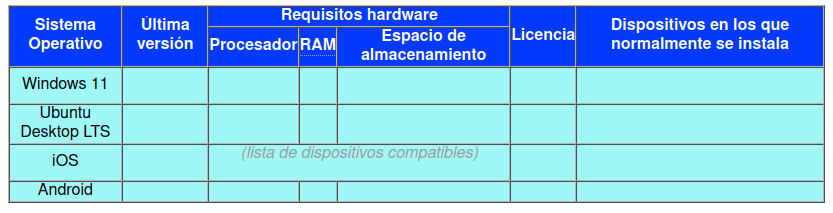
\includegraphics[scale=0.55]{tabla-so.png}
    \caption{Tabla para rellenar sobre SOs}
\end{figure}

\subsubsection{Solución}
En este punto vamos a ver información básica sobre los diferentes sistemas operativos más extendidos en la actualidad. En la siguiente figura se muestra una tabla con toda la información pedida.

Dentro de la sección de requisitos de hardware se incluirán los requisitos mínimos, no los recomendados. El colo de la tabla también puede diferir de la que se muestra en el enunciado, pero el contenido es el solicitado.

\begin{figure}[ht]
    \centering
    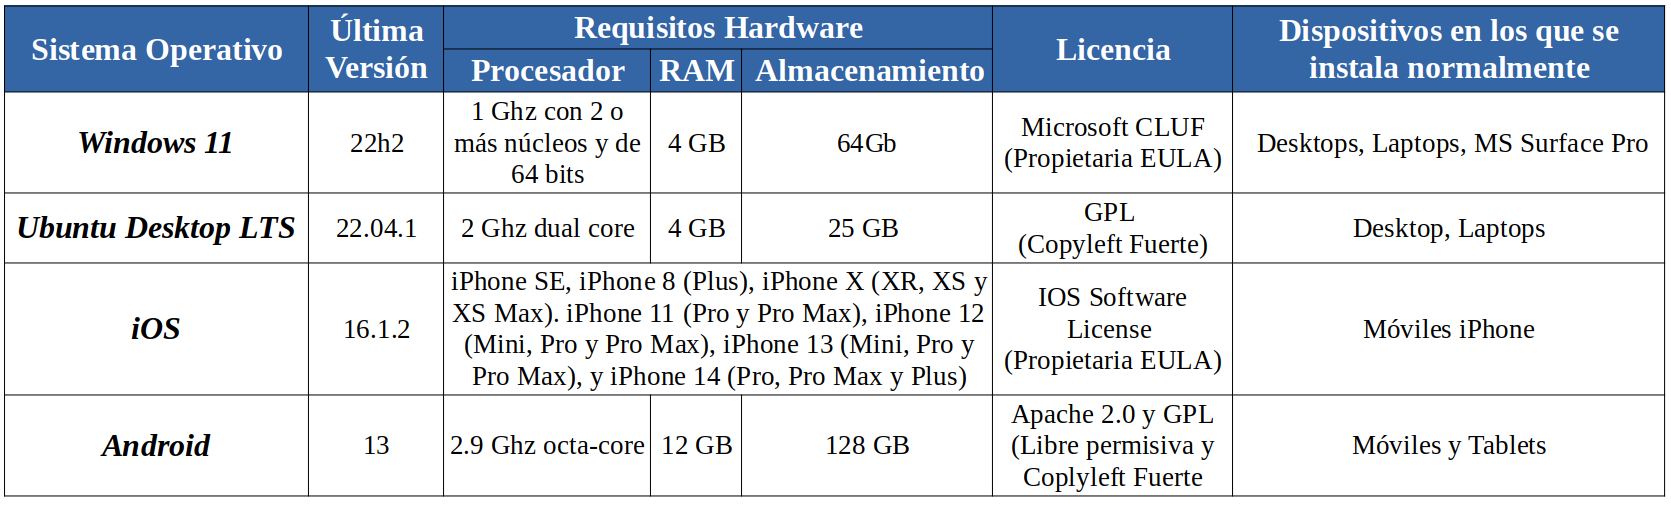
\includegraphics[scale=0.35]{tabla-so-completa.png}
    \caption{Tabla características SOs}
\end{figure}

Para el apartado de \textbf{Android}, se ha incluido el teléfono \textbf{Samsung Galaxy S21 Ultra}. Actualmente no hay móviles que salgan con Android 13, ya que esta versión es muy reciente (Agosto de 2022), pero si hay muchos que se han actualizado a esta versión desde la versión 12, este Samsung es uno de ellos.

\subsection{Actividad 4: Arquitectura Interna de un Sistema Operativo}
Explica en qué consisten las siguientes arquitecturas de sistemas operativos:

\begin{itemize}
    \item Monolítica.
    \item Microkernel.
    \item Híbrida.
\end{itemize}

Indica, además, un ejemplo de SO para cada arquitectura.

\subsubsection{Solución}
En este punto vamos a explicar diferentes arquitecturas de Kernel, explicando un poco sus características y poniendo un ejemplo de un sistema operativo que las use.

\begin{itemize}
    \item \textbf{Arquitectura Monolítica}

    En este tipo de arquitectura \textbf{todas las funciones} se implementan \textbf{dentro del núcleo}, es decir, todos los servicios del sistema operativo se ejecutan dentro de hilo principal del Kernel. También se incluyen dentro del núcleo \textbf{todos los drivers} necesarios para que funcionen los diferentes dispositivos. Este tipo de arquitectura ha sido empleado tradicionalmente por los sistemas tipo Unix. \cite{wiki04}

    Algunos desarrolladores, como Ken Thompson, mantienen que es ``más fácil de implementar'' que otras arquitecturas, como los microkernels, aunque son núcleos más difíciles de mantener, principalmente por la dependencia entre los componentes del sistema. \cite{wiki03}

    Algunos ejemplos de este tipo de kernel son los sistemas \textbf{GNU/Linux}, \textbf{BSD} (FreeBSD, OpenBSD, NetBSD), y los sistemas basados en \textbf{UNIX System V}, como \textbf{Solaris} o \textbf{HP-UX}. El sistema \textbf{MS-DOS} también usaba esta arquitectura.

    \item \textbf{Microkernel}

    En este tipo de arquitectura, muchas de las \textbf{funcionalidades} que históricamente se implementaban dentro del kernel se mueven \textbf{fuera de éste}, en un conjunto de ``\textbf{servidores}'' que se comunican a través de un kernel con el mínimo posible de código. Estos servidores, al contrario que en otros kernel, se ejecutan en el \textbf{espacio de usuario} en vez de en el \textbf{espacio de sistema}, manteniéndose en éste solo lo imprescindible, como el \textbf{IPC} (Inter Process Comunitacion), que permite la comunicación entre los diferentes procesos. \cite{wiki03}

    Esta arquitectura tiene varias \textbf{ventajas} sobre la monolítica, como que son \textbf{más fácil de mantener}, los \textbf{parches} se pueden \textbf{testear} en instancias separadas y son más rápidos de desarrollar. Pero también tiene algunos \textbf{inconvenientes}, como que los \textbf{programas necesitan más memoria} para poder ejecutarse, la \textbf{gestión de procesos} es más \textbf{compleja}, y el rendimiento es menor que en los kernel monolíticos. \cite{wiki03}

    Algunos ejemplos de sistemas operativos con microkernel son \textbf{AmigaOS}, \textbf{Minix} y 	\textbf{HarmonyOS}, entre otros.

    \item \textbf{Arquitectura Híbrida}

    Estos tipos de kernel son \textbf{similares} a los \textbf{microkernel}, con la diferencia de que \textbf{incluyen más funcionalidades} dentro de \textbf{núcleo} para mejorar el rendimiento de éste, combinando, por así decirlo, las arquitecturas monolítica y microkernel. La idea es tener una estructura similar a un microkernel, pero implementando esa estructura de forma monolítica, así, no tienen los beneficios de tener los servicios del SO en el espacio de usuario, pero tampoco tienen la sobrecarga en el paso de mensajes que esto puede ocasionar, siendo en este aspecto más similar a un kernel monolítico. \cite{wiki05}

    El ejemplo más conocido de este tipo de kernel son los sistemas \textbf{Microsoft Windows}, que desde la versión \textbf{Windows NT} se lleva empleando en todos sus sistemas operativos, incluido la ultima versión, \textbf{Windows 11}. También hay otros sistemas que emplean este tipo de arquitectura, como \textbf{BeOS}, \textbf{Netware} o \textbf{ReactOS}.


\end{itemize}


% Bibliography

\newpage
\bibliography{citas}
\bibliographystyle{unsrt}

\end{document}